\chapter{Repere teoretice în inteligența artificială și calculul neuromorfic}
\label{ch:fundamente_teoretice}

\section{Modele de învățare automată și rețele artificiale de a doua generație}

Prima parte a capitolului este dedicată analizei fundamentelor teoretice care stau la baza modelelor computaționale utilizate în prezenta lucrare. Se va realiza o trecere în revistă a evoluției de la algoritmii clasici de învățare automată, bazați pe statistica matematică, până la arhitecturile complexe de învățare profundă de a doua generație, evidențiind principiile lor de funcționare, avantajele structurale și limitările care au condus la necesitatea dezvoltării rețelelor neuromorfice.

\subsection*{Mașini cu suport vectorial (SVM)}
Înainte de ascensiunea rețelelor neuronale adânci, mașinile cu vectori suport (\textit{Support Vector Machines} -- SVM) au reprezentat standardul de performanță în clasificarea supervizată, fiind fundamentate pe principiile teoriei statistice a învățării, formalizată de Vapnik și Chervonenkis \cite{vapnik1995}. Spre deosebire de abordările bazate pe rețele neuronale, SVM-ul nu necesită o arhitectură ierarhică adâncă și se dovedește extrem de eficient inclusiv în spații de trăsături de dimensionalitate ridicată, gestionând stabil seturi de date relativ mici.

Principiul fundamental al SVM constă în identificarea unui \textbf{hiperplan de separare optim} în spațiul trăsăturilor, definit ca hiperplanul care maximizează \textbf{marginea} (\textit{margin}) dintre clasele de date. Formal, pentru un set de date $\{(\mathbf{x}_i, y_i)\}_{i=1}^{N}$, cu $y_i \in \{-1, +1\}$, se caută vectorul de ponderi $\mathbf{w}$ și pragul $b$ care satisfac relația \eqref{eq:svm_hard}:
\begin{equation}
	\label{eq:svm_hard}
	\min_{\mathbf{w}, b}\ \frac{1}{2}\|\mathbf{w}\|^2 \quad \text{a.î.} \quad y_i(\mathbf{w}^\top \mathbf{x}_i + b) \geq 1, \quad \forall i = 1, \dots, N.
\end{equation}

Vectorii de antrenare situați pe granița marginii (la distanța minimă față de hiperplan) poartă denumirea de vectori suport (\textit{support vectors}) și sunt singurii care influențează poziția hiperplanului de decizie, conferind modelului robustețe la \textit{outlieri}. Pentru datele neseparabile liniar, modelul introduce variabilele de relaxare (\textit{slack variables}) $\xi_i \geq 0$ și parametrul de regularizare $C$, controlând prin relația \eqref{eq:svm_soft} compromisul dintre maximizarea marginii și toleranța la erori (\textit{soft-margin SVM}):
\begin{equation}
	\label{eq:svm_soft}
	\min_{\mathbf{w}, b, \boldsymbol{\xi}}\ \frac{1}{2}\|\mathbf{w}\|^2 + C\sum_{i=1}^{N}\xi_i.
\end{equation}

Prin intermediul \textbf{trucului kernel} (\textit{kernel trick}), SVM-ul poate opera implicit în spații de trăsături de dimensionalitate foarte mare fără a calcula explicit transformarea neliniară. Înlocuirea produsului scalar cu o funcție dedicată, precum \textbf{Kernelul RBF} (\textit{Radial Basis Function}): $K(\mathbf{x}_i, \mathbf{x}_j) = \exp\left(-\gamma \|\mathbf{x}_i - \mathbf{x}_j\|^2\right)$, permite separarea unor distribuții complexe. Extensia la clasificare multiclasă (necesară pentru cele 7 emoții din setul CK+) se realizează prin strategia \textit{One-vs-One}. Folosind biblioteca \texttt{LIBSVM}, algoritmul antrenează un număr de $\frac{7 \times (7 - 1)}{2} = 21$ de clasificatori binari independenți, decizia finală fiind determinată prin cuplarea probabilităților parțiale (scalarea Platt) într-o distribuție probabilistică unitară.

În cadrul acestei lucrări, SVM-ul este utilizat atât ca model de referință \textit{baseline} aplicat direct pe pixeli bruți, cât și drept clasificator final în pipeline-ul propus, primind vectorii de trăsături spațio-temporale extrași de rețeaua SNN. Această decuplare între extracția nesupervizată (prin STDP) și clasificare urmează o metodologie consacrată în literatură \cite{kheradpisheh2018stdp}, permițând evaluarea izolată a calității reprezentărilor învățate de rețeaua neuronală cu impulsuri.

\subsection*{Învățarea automată și rețele neuronale artificiale (ANN)}

Deși modelele matematice riguroase precum SVM oferă garanții teoretice solide, limitările lor în extragerea automată a ierarhiilor de trăsături din date brute au propulsat o altă paradigmă: învățarea computațională bazată pe rețele neuronale artificiale (ANN). Concepute ca o abstractizare simplificată a rețelelor biologice, însă simplificate structural pentru a fi compatibile cu hardware-ul convențional, ANN-urile trec de la geometria hiperplanelor la structuri ierarhice stratificate.

Funcționarea unei rețele neuronale standard se bazează pe transmiterea in\-for\-ma\-ți\-ei printr-o ierarhie de straturi compuse din unități de procesare elementare. Fiecare neuron artificial realizează o transformare a datelor de intrare în două etape succesive. În prima fază, se calculează o combinație liniară a semnalelor de intrare, unde fiecare contribuție este ajustată prin intermediul unor coeficienți numiți ponderi (sau greutăți). Rolul acestora este de a amplifica sau atenua importanța fiecărui semnal în procesul decizional. Matematic, această sumă ponderată, la care se adaugă un termen de polarizare (\textit{bias}), este exprimată prin relația \eqref{eq:suma_ponderata}:

\begin{equation}
\label{eq:suma_ponderata}
z = \sum_{i=1}^{n} w_i x_i + b,
\end{equation}
unde $x_i$ reprezintă intrările sistemului, $w_i$ sunt ponderile asociate, iar $b$ este termenul de \textit{bias}. În a doua etapă, pentru a introduce neliniaritatea necesară modelării unor fenomene complexe, rezultatul $z$ este procesat de o funcție de activare $\sigma$. Valoarea finală de ieșire a neuronului, $y$, este definită de ecuația \eqref{eq:activare}, întregul proces fiind ilustrat schematic în Figura \ref{fig:neuron_artificial}:

\begin{equation}
\label{eq:activare}
y = \sigma(z) = \sigma \left( \sum_{i=1}^{n} w_i x_i + b \right).
\end{equation}

\begin{figure}[htbp]
    \centering
    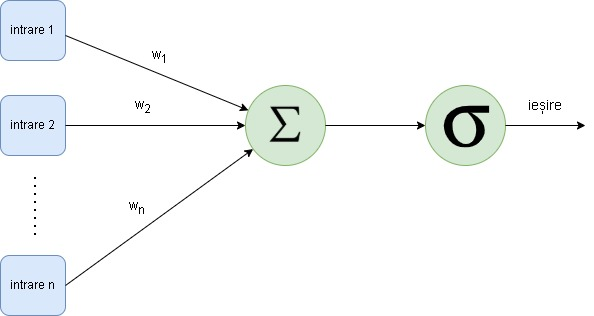
\includegraphics[width=0.6\textwidth]{images/neuron_artificial.jpg} 
    \caption{Reprezentarea schematică a unui neuron artificial: procesarea intrărilor prin ponderare și aplicarea funcției de activare.}
    \label{fig:neuron_artificial}
\end{figure}

Deși aceste rețele au demonstrat performanțe remarcabile, ele prezintă limitări inerente. Utilizarea valorilor numerice continue, conform modelului descris în ecuația \eqref{eq:activare}, forțează sistemul să realizeze calcule intensive în mod constant. Acest aspect conduce la un cost computațional ridicat și la un consum energetic substanțial, care rămâne invariant indiferent de relevanța sau densitatea informației procesate.

\subsection*{Rețele neuronale convoluționale (CNN)}
Rețelele neuronale convoluționale (\textit{Convolutional Neural Networks} -- CNN) reprezintă o categorie specializată de arhitecturi ANN, proiectate explicit pentru procesarea datelor cu structură spațială, cum ar fi imaginile sau secvențele video. Spre deosebire de rețelele complet conectate (\textit{fully connected}), care tratează fiecare pixel ca o intrare independentă, CNN-urile exploatează corelațiile locale dintre pixelii vecini prin intermediul operației de convoluție, reducând drastic numărul de parametri și conferind invarianță la translație.

Operația de convoluție constituie nucleul funcțional al acestor arhitecturi. Un filtru (\textit{kernel}) de dimensiune redusă $k \times k$ este aplicat glisant pe întreaga suprafață a imaginii de intrare, calculând la fiecare poziție $(x,y)$ produsul scalar dintre valorile locale și ponderile filtrului, după cum reiese din ecuația \eqref{eq:convolutie}:
\begin{equation}
	\label{eq:convolutie}
	\text{FeatureMap}(x, y) = \sum_{i=0}^{k-1} \sum_{j=0}^{k-1} I(x+i, y+j) \cdot W(i, j) + b,
\end{equation}
unde $I$ reprezintă imaginea de intrare, $W$ este matricea de ponderi a filtrului, iar $b$ este termenul de \textit{bias}. Rezultatul acestei operații este o \textbf{hartă de trăsături} (\textit{feature map}), care codifică prezența unui anumit tipar vizual (de exemplu, o margine orizontală sau un colț) în diverse regiuni ale imaginii.

O arhitectură CNN tipică este compusă din mai multe tipuri de straturi:
\begin{itemize}[noitemsep]
	\item \textbf{Straturi convoluționale}: Aplică un set de filtre antrenabile, generând hărți de trăsături pentru tipare de complexitate crescândă pe măsura adâncirii rețelei.
	\item \textbf{Straturi de activare}: Introduc neliniaritatea necesară, funcția \textit{ReLU} (\textit{Rectified Linear Unit}), $\sigma(z) = \max(0, z)$, fiind cea mai frecvent utilizată în arhitecturile moderne datorită eficienței sale computaționale și comportamentului stabil la antrenare.
	\item \textbf{Straturi de pooling}: Reduc rezoluția spațială a hărților de trăsături prin agregarea valorilor dintr-o vecinătate locală (ex. \textit{MaxPooling}, \textit{AvgPooling}), conferind robustețe la mici variații de poziție.
	\item \textbf{Straturi complet conectate (Fully Connected)}: Situate la finalul rețelei, realizează maparea vectorului de trăsături extrase către spațiul claselor de ieșire.
\end{itemize}

Antrenarea CNN-urilor se realizează prin algoritmul de \textit{backpropagation}, care propagă eroarea de la stratul de ieșire către straturile anterioare și actualizează ponderile filtrelor prin metoda gradientului descendent. Gradul de expresivitate al acestor rețele crește exponențial cu adâncimea lor, arhitecturi profunde precum ResNet \cite{he2016} sau VGG \cite{simonyan2015very} reușind să extragă trăsături semantice de nivel înalt.

ResNet, utilizat ca extractor de trăsături spațiale, introduce mecanismul \textit{residual connections} (conexiuni reziduale), prin care ieșirea unui bloc de straturi este adunată cu intrarea sa originală în ecuația \eqref{eq:resnet}:
\begin{equation}
	\label{eq:resnet}
	\mathbf{y} = \mathcal{F}(\mathbf{x}, \{W_i\}) + \mathbf{x}.
\end{equation}
Această abordare rezolvă problema dispariției gradientului (\textit{vanishing gradient}) în rețelele adânci, permițând antrenarea eficientă a arhitecturilor cu zeci sau sute de straturi.

\subsection*{Rețele recurente și LSTM}
Rețelele neuronale complet conectate și CNN-urile tratează fiecare intrare ca independentă, ignorând orice dependență temporală sau secvențială. Pentru sarcinile în care ordinea elementelor este esențială -- recunoașterea vorbirii, analiza seriilor de timp sau recunoașterea expresiilor faciale dintr-o secvență video -- această limitare devine critică.

\textbf{Rețelele neuronale recurente} (\textit{Recurrent Neural Networks} -- RNN) adresează această problemă prin introducerea unei bucle de feedback: ieșirea neuronului la pasul temporal $t$ este transmisă ca intrare suplimentară la pasul $t+1$, permițând rețelei să mențină o \textbf{stare ascunsă} (\textit{hidden state}) $\mathbf{h}_t$ care codifică informația acumulată din pașii anteriori. după cum se poate observa în ecuația \eqref{eq:rnn}:
\begin{equation}
	\label{eq:rnn}
	\mathbf{h}_t = \sigma\left(W_h \mathbf{h}_{t-1} + W_x \mathbf{x}_t + b\right).
\end{equation}

Cu toate acestea, RNN-urile clasice suferă de problema dispariției sau explozia gradientului în secvențe lungi: gradientul propagat înapoi prin multe etape temporale tinde fie să se anuleze (împiedicând învățarea dependențelor pe termen lung), fie să crească exponențial (destabilizând antrenamentul).

\textbf{Rețelele LSTM} (\textit{Long Short-Term Memory}), introduse de Hochreiter și Schmidhuber \cite{hochreiter1997}, rezolvă această problemă printr-un mecanism explicit de \textbf{memorie gestionată prin porți} (\textit{gated memory}). Unitatea LSTM menține două stări: starea celulei $\mathbf{c}_t$ (memoria pe termen lung) și starea ascunsă $\mathbf{h}_t$ (memoria pe termen scurt), actualizate conform componentelor descrise în Tabela~\ref{tab:lstm_components}.

\begin{table}[htbp]
	\centering
	\caption{Componentele structurale ale unei unități LSTM și ecuațiile lor matematice.}
	\label{tab:lstm_components}
	\small
	\begin{tabular}{@{} l p{6.5cm} l @{}}
		\hline
		\textbf{Componentă} & \textbf{Rol funcțional} & \textbf{Ecuație de calcul} \\ \hline
		\rule{0pt}{3ex}Poarta de uitare & Decide ce informație din starea anterioară a celulei trebuie eliminată. & $\displaystyle \mathbf{f}_t = \sigma\left(W_f \cdot [\mathbf{h}_{t-1}, \mathbf{x}_t] + b_f\right)$ \\[1.5ex]
		Poarta de intrare & Determină ce proporție din informația nouă va fi transmisă mai departe. & $\displaystyle \mathbf{i}_t = \sigma\left(W_i \cdot [\mathbf{h}_{t-1}, \mathbf{x}_t] + b_i\right)$ \\[1.5ex]
		Starea candidată & Creează un vector cu noile valori potențiale ce pot fi adăugate în starea celulei. & $\displaystyle \tilde{\mathbf{c}}_t = \tanh\left(W_c \cdot [\mathbf{h}_{t-1}, \mathbf{x}_t] + b_c\right)$ \\[1.5ex]
		Poarta de ieșire & Determină ce parte din starea celulei este propagată ca ieșire curentă. & $\displaystyle \mathbf{o}_t = \sigma\left(W_o \cdot [\mathbf{h}_{t-1}, \mathbf{x}_t] + b_o\right)$ \\[1ex] \hline
	\end{tabular}
\end{table}

Actualizarea stărilor se realizează conform relațiilor \eqref{eq:lstm_c_u_update}:
\begin{equation}
	\label{eq:lstm_c_u_update}
	\mathbf{c}_t = \mathbf{f}_t \odot \mathbf{c}_{t-1} + \mathbf{i}_t \odot \tilde{\mathbf{c}}_t, \qquad \mathbf{h}_t = \mathbf{o}_t \odot \tanh(\mathbf{c}_t),
\end{equation}
unde $\odot$ denotă produsul element-cu-element (Hadamard). Prin această arhitectură, LSTM-ul poate reține în mod selectiv informații relevante pe durate arbitrar de lungi, ignorând zgomotul temporal.

Acest mecanism permite modelarea tranzițiilor musculare faciale fine de la faza neutră la apexul emoției. Cu toate acestea, la fel ca toate arhitecturile de învățare profundă din cea de-a doua generație, modelele convoluționale și recurente se confruntă cu două limitări structurale majore: dependența critică de volume masive de date adnotate și costul computațional exorbitant. Pe de o parte, capacitatea de generalizare a acestor rețele este strâns legată de existența unor seturi de date uriașe, curate și etichetate manual, o resursă extrem de costisitoare și dificil de obținut în cazul analizelor de nișă (cum sunt secvențele video dinamice pentru emoții). Pe de altă parte, procesarea continuă și sincronă a matricilor matematice forțează rularea a miliarde de operații în virgulă mobilă (\textit{floating-point operations}) per cadru. Acest aspect generează un consum energetic masiv și o latență incompatibilă cu sistemele încapsulate, menținând o barieră tehnologică rigidă în calea implementării pe dispozitive cu resurse limitate.

\section{Trecerea de la ANN la Spiking Neural Networks (SNN)}

Limitările computaționale și energetice menționate anterior au impus tranziția către o nouă paradigmă: rețelele neuronale cu impulsuri (\textit{Spiking Neural Networks} - SNN). Considerate a treia generație a rețelelor neuronale, SNN-urile se apropie mult mai mult de mecanismele fiziologice ale creierului, înlocuind valorile continue cu impulsuri discrete de joasă energie, numite \textit{spikes} \cite{tavanaei2019deep}.

Spre deosebire de modelele clasice, SNN-urile adoptă o abordare bazată pe evenimente (\textit{event-driven}), caracterizată printr-o activare rară (\textit{sparse activation}), așa cum se poate observa în Figura \ref{fig:ann_vs_snn}. În acest context, neuronii procesează evenimente distribuite temporal, activându-se doar atunci când stimulii recepționați ating un anumit prag critic. Această proprietate elimină necesitatea calculelor redundante în perioadele de inactivitate, optimizând consumul de resurse \cite{falez2019multi}. Mai mult, natura asincronă a acestor rețele facilitează paralelizarea proceselor, oferind avantaje clare de viteză pe hardware neuromorfic dedicat \cite{bing2019supervised}.

\begin{figure}[htbp]
	\centering
	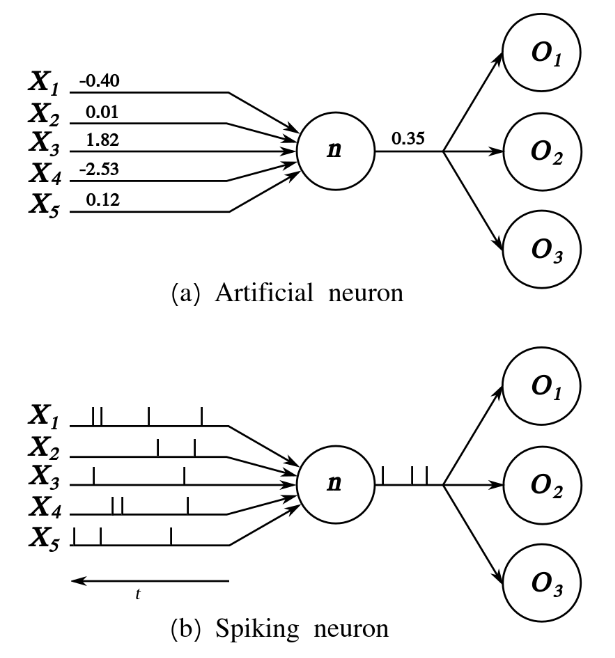
\includegraphics[width=0.45\textwidth]{figures/artificial_vs_spiking_neuron.png}
	\caption{Comparație între un neuron artificial și un neuron cu impulsuri (\textit{spiking neuron}). Sursă: \cite{elassal2024}.}
	\label{fig:ann_vs_snn}
\end{figure}

\section{Modelarea matematică a neuronului cu impulsuri}

Spre deosebire de modelele generațiilor anterioare, rețelele neuronale cu impulsuri (SNN) utilizează ca unitate fundamentală de comunicare fluxuri de impulsuri discrete, cunoscute sub denumirea de \textit{spike trains}. Fiecare impuls reprezintă un potențial de acțiune, o descărcare electrică de scurtă durată care transportă informația prin rețea, imitând fidel procesele electro-chimice din creierul uman.

Mecanismul de funcționare al unui neuron de tip \textit{spiking} este definit prin in\-te\-rac\-ți\-u\-nea dintre potențialul de membrană și un prag de activare (\textit{firing threshold}). Procesul poate fi sintetizat în patru etape critice:

\begin{itemize}
    \item \textbf{Integrarea și acumularea:} Neuronul recepționează semnale de intrare prin sinapse și le cumulează în timp, ceea ce determină o creștere incrementală a potențialului de membrană.
    \item \textbf{Declanșarea (\textit{Firing}):} În momentul în care potențialul acumulat atinge sau depășește valoarea pragului critic stabilit, neuronul generează un impuls de ieșire (\textit{spike}).
    \item \textbf{Resetarea:} Imediat după generarea impulsului, potențialul de membrană revine la o valoare de bază, numită stare de repaus (\textit{resting state}).
    \item \textbf{Perioada refractară:} Urmează un scurt interval de timp în care neuronul devine insensibil la noile impulsuri primite, indiferent de intensitatea acestora, permițând refacerea echilibrului ionic.
\end{itemize}

Evoluția temporală a acestor etape și modul în care potențialul de membrană reacționează la stimulii externi sunt ilustrate în Figura \ref{fig:dinamica_membrana}.

\begin{figure}[htbp]
    \centering
    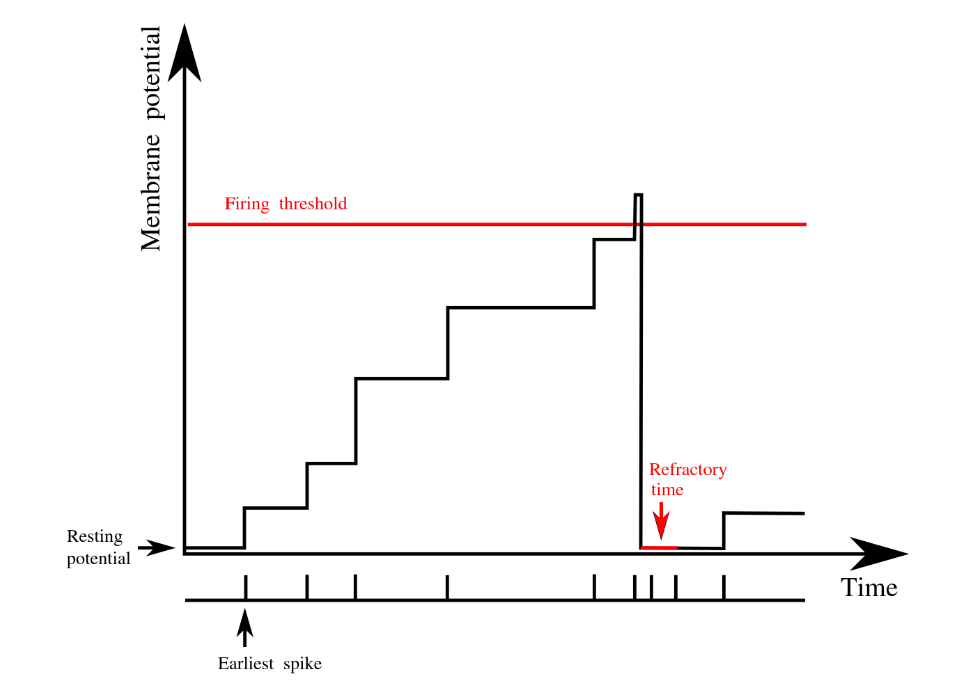
\includegraphics[width=0.75\textwidth]{figures/dinamica_membranei.png}
    \caption{Evoluția potențialului de membrană al unui neuron de tip \textit{spiking} ca răspuns la un tren de impulsuri de intrare. Se observă fazele de acumulare, atingerea pragului critic, generarea impulsului și perioada de resetare. Sursă: \cite{elassal2024}.}
    \label{fig:dinamica_membrana}
\end{figure}

\subsection*{Modele de neuroni: de la biologie la eficiență hardware}
În literatura de specialitate, există o varietate de modele matematice care descriu acest comportament, prezentând un compromis direct între plauzibilitatea biologică și complexitatea computațională \cite{izhikevich2004}.

\begin{enumerate}
    \item \textbf{Modelul Hodgkin-Huxley \cite{hodgkin1952}:} Este unul dintre cele mai detaliate modele biofizice, utilizând un sistem de ecuații diferențiale neliniare pentru a descrie dinamica canalelor ionice (sodiu și potasiu). Deși oferă o acuratețe biologică ridicată, costul computațional necesar pentru simularea acestuia îl face extrem de dificil de implementat în sisteme hardware neuromorfice la scară largă.
    \item \textbf{Modelul Integrate-and-Fire (IF) \cite{burkitt2006}:} Reprezintă varianta cea mai simplificată și eficientă din punct de vedere algoritmic. În ciuda arhitecturii sale elementare, modelul IF s-a dovedit a fi un instrument robust în aplicațiile de învățare vizuală și recunoaștere a formelor, fiind preferat în designul sistemelor de tip \textit{edge AI}.
\end{enumerate}

Modelul IF descrie evoluția potențialului de membrană $V_m(t)$ ca o acumulare liniară a ponderilor sinaptice asociate impulsurilor recepționate. Dinamica sistemului, guvernată de capacitatea membranei $c_m$, este exprimată prin relația \eqref{eq:if_dinamica}:

\begin{equation}
\label{eq:if_dinamica}
c_m V_m(t) = V_r + \sum_{i \in E} w_i f_s(t - t_i),
\end{equation}
unde $V_r$ reprezintă potențialul de repaus al membranei; $E$ constituie setul de impulsuri de intrare; $w_i$ este ponderea sinaptică (greutatea) asociată celui de-al $i$-lea impuls; $t_i$ reprezintă coordonata temporală a recepționării impulsului; iar $f_s$ este funcția nucleu (\textit{spike kernel}), definită conform relației \eqref{eq:spike_kernel}:

\begin{equation}
\label{eq:spike_kernel}
f_s(x) = 
\begin{cases} 
1, & \text{dacă } x \geq 0 \\
0, & \text{în caz contrar}
\end{cases}.
\end{equation}

Regula de actualizare a stării neuronului impune ca atunci când potențialul de membrană depășește pragul $V_{th}$, să aibă loc descărcarea, urmată de resetarea po\-ten\-ți\-a\-lu\-lui, așa cum reiese din relația \eqref{eq:reset_rule}:

\begin{equation}
\label{eq:reset_rule}
V_m(t) \leftarrow V_r, \quad \text{pentru} \quad V_m(t) \geq V_{th}(t).
\end{equation}

Această abordare matematică permite procesarea eficientă a datelor asincrone, fiind ideală pentru sarcini care implică o dinamică temporală complexă, cum este identificarea emoțiilor în secvențe video.

\section{Filtrarea bio-inspirată On/Off}

Înainte ca pixelii bruți ai imaginilor sau cadrelor video să fie transformați în impulsuri temporale, este necesară o etapă de preprocesare capabilă să extragă contrastele spațiale locale și să elimine redundanța informațională. În sistemul vizual biologic, dar și în cazul senzorilor de viziune bazați pe evenimente (DVS), această funcție este îndeplinită de celulele ganglionare retiniene cu structură de tip centru-periferie (\textit{center-surround}). 

Pentru a simula digital acest comportament, se aplică o filtrare liniară bazată pe modelul \textbf{DoG} (\textit{Difference of Gaussians})\cite{rodieck1965quantitative}, care extrage gradienții de contrast prin diferența a două funcții Gaussiene cu deviații standard distincte: una pentru regiunea centrală ($\sigma_{center}$) și una pentru regiunea înconjurătoare ($\sigma_{surround}$). Valoarea rezultată $v$ în urma convoluției imaginii cu filtrul DoG este apoi separată în două canale complet independente, dublând dimensiunea pe adâncime (\textit{depth}) a tensorului de date:

\begin{itemize}[noitemsep]
	\item \textbf{Canalul ON:} Reține exclusiv valorile pozitive ale contrastului, simulând activarea celulelor sensibile la tranziția de la întuneric la lumină (relația \eqref{eq:dog_on}):
	\begin{equation}
		\label{eq:dog_on}
		I_{ON} = \max(0, v).
	\end{equation}
	\item \textbf{Canalul OFF:} Reține magnitudinea valorilor negative (inversate), simulând celulele sensibile la tranziția de la lumină la întuneric (relația \eqref{eq:dog_off}):
	\begin{equation}
		\label{eq:dog_off}
		I_{OFF} = \max(0, -v).
	\end{equation}
\end{itemize}

Pentru a preveni propagarea zgomotului de fond de joasă intensitate și a menține caracterul selectiv (\textit{sparse}) al rețelei, se introduce un parametru de prag critic (\textit{cutoff}). Orice valoare de contrast care nu depășește acest nivel de tăiere este anulată, fiind păstrate doar marginile și formele cu o relevanță semantică ridicată.

Odată realizată separarea structurală în fluxuri ON și OFF, amplitudinile rezultate prezintă scale dinamice, variabile de la un cadru la altul. Deoarece funcția de codificare prin latență (descrisă în secțiunea următoare \ref{sc:codificare}) necesită o intrare strict delimitată în intervalul normat $[0, 1]$, se impune aplicarea modulului \textbf{MaxScaling}. Rolul acestei tehnici este de a normaliza valorile din tensorul filtrat, raportându-le dinamic la valoarea maximă absolută identificată în eșantionul curent, conform relației \eqref{eq:max_scaling}:

\begin{equation}
	\label{eq:max_scaling}
	x_{scaled} = \frac{x}{\max(X)}.
\end{equation}
Această etapă de aliniere garantează că pixelul cu cel mai pronunțat contrast din scenă va fi mapat perfect pe valoarea unitară ($1.0$), devenind ulterior primul impuls generat în timp, facilitând astfel funcționarea corectă a codificării temporale.

\section{Codificarea informației neurale}
\label{sc:codificare}

Întrucât rețelele neuronale cu impulsuri procesează informația sub formă de evenimente discrete, transformarea datelor de intrare (semnale analogice sau valori digitale continue) în trenuri de impulsuri (\textit{spike trains}) reprezintă o etapă fundamentală. În contextul prezentei lucrări, datele de intrare sunt prezentate neuronilor secvențial, eșantion cu eșantion. Fiecare stimul este menținut pentru un interval temporal definit, cunoscut sub numele de perioadă de expunere sau $t_{exposition}$ \cite{falez2019}. 

Deși există numeroase scheme de codificare, acestea pot fi clasificate în două categorii majore, în funcție de modul în care informația este reprezentată în raport cu timpul.

\subsection*{Rate Coding}
Codificarea prin rată corelează intensitatea stimulului de intrare $x \in [0, 1]$ cu frecvența de apariție a impulsurilor. Din punct de vedere computațional, acest proces este modelat printr-un proces stochastic Poisson \cite{gerstner2002spiking}. Probabilitatea ca un neuron $i$ să emită un impuls ($S_i = 1$) într-un interval de timp discret foarte mic $\Delta t$ este proporțională cu valoarea semnalului de intrare, aspect ilustrat în ecuația \eqref{eq:impuls_rate_coding}:

\begin{equation}
\label{eq:impuls_rate_coding}
P(S_i[t] = 1) = x \cdot \Delta t,
\end{equation}
unde $x$ reprezintă intensitatea stimulului (rata de descărcare dorită), $\Delta t$ este pasul de simulare temporală, $S_i[t] \in \{0, 1\}$ este variabila Bernoulli care indică prezența unui impuls la momentul $t$.

Deși este robustă, codificarea prin rată prezintă limitări semnificative în ceea ce privește viteza de procesare. Pentru a obține o reprezentare precisă a valorii codificate, neuronii post-sinaptici trebuie să integreze un număr ridicat de impulsuri pe o durată extinsă \cite{guo2021}. Acest fenomen introduce o latență inerentă în rețea, deoarece decizia este condiționată de acumularea unei statistici suficiente a impulsurilor.

\subsection*{Temporal Coding}
Spre deosebire de codificarea prin rată, metodele temporale utilizează momentul precis al apariției impulsurilor (\textit{timestamps}) pentru a reprezenta informația, oferind o eficiență energetică și temporală superioară.

\subsubsection{Rank Order Coding}
Codificarea prin ordinea rangului \cite{thorpe1998} se bazează pe premisa că ordinea în care neuronii dintr-o populație declanșează impulsuri poartă informația esențială \cite{delorme2001}. Neuronii care primesc stimuli de intensitate ridicată tind să se activeze înaintea celor stimulați slab. O formă simplificată de reprezentare a acestui impact, independentă de modelul de neuron utilizat, este redată de ecuația \eqref{eq:rank_order}:

\begin{equation}
\label{eq:rank_order}
f_{in}(x_i) = r(x_i) \times \frac{1}{n},
\end{equation}
unde $x_i$ este valoarea de intrare, $n$ reprezintă numărul total de conexiuni, iar $r(x_i)$ reprezintă rangul (poziția în ordine descrescătoare) al valorii $x_i$ în setul de intrări.

\subsubsection{Latency Coding}
Codificarea prin latență \cite{gollisch2008} reprezintă intensitatea stimulului prin intervalul de timp scurs până la primul impuls. Un stimul puternic va genera un răspuns rapid (latență mică), în timp ce un stimul slab va întârzia activarea neuronului. Relația de inversă proporționalitate între intensitatea $x$ și momentul declanșării este formalizată prin ecuația \eqref{eq:latency}:

\begin{equation}
\label{eq:latency}
f_{in}(x) = (1.0 - x) \times t_{exposition}.
\end{equation}

Această abordare este deosebit de eficientă pentru procesarea video, deoarece permite rețelei să reacționeze extrem de rapid la schimbările semnificative din câmpul vizual, procesând prioritar cele mai relevante informații.

\section{Mecanisme de învățare și plasticitate sinaptică}

Capacitatea de procesare a informației în cadrul rețelelor SNN rezidă în conexiunile sinaptice dintre neuroni. \textbf{Plasticitatea sinaptică} reprezintă proprietatea fundamentală a acestor conexiuni de a-și modifica intensitatea (ponderea sinaptică) în funcție de tiparele activității neuronale și de regulile de învățare aplicate. Din punct de vedere funcțional, ponderile sinaptice modulează probabilitatea de declanșare a neuronului post-sinaptic: o pondere ridicată amplifică contribuția unui impuls recepționat, în timp ce o pondere scăzută atenuează impactul acestuia asupra po\-ten\-ți\-a\-lu\-lui de membrană.

Antrenarea acestor rețele presupune ajustarea sistematică a ponderilor și a pragurilor de activare pentru a permite sistemului să identifice trăsături relevante în datele de intrare. În literatura de specialitate, metodele de antrenare a SNN-urilor pot fi clasificate în trei paradigme majore.

\subsection*{Conversia ANN în SNN}
Această abordare presupune antrenarea prealabilă a unei rețele neuronale artificiale (ANN) convenționale, utilizând algoritmi standard precum \textit{Backpropagation}, urmată de transferul și adaptarea ponderilor învățate către o arhitectură SNN echivalentă \cite{kugele2020}. 

Procesul de conversie urmărește conservarea funcționalității și a performanței rețelei originale prin scalarea ponderilor și ajustarea acestora la intervalul dinamic specific modelului de neuron cu impulsuri ales. Deși această metodă oferă rezultate competitive și permite utilizarea infrastructurii software existente pentru \textit{Deep Learning}, ea prezintă limitări critice:
\begin{itemize}
    \item Necesită resurse computaționale ridicate pentru etapa inițială de antrenare a ANN-ului.
    \item Implică procese post-conversie complexe, precum normalizarea ponderilor și echilibrarea pragurilor (\textit{threshold balancing}).
    \item Nu exploatează pe deplin avantajele temporale native ale SNN-urilor în timpul procesului de învățare.
\end{itemize}

\subsection*{Spiking back-propagation}
O altă metodă supervizată constă în adaptarea directă a algoritmului \textit{Backpropagation} pentru domeniul impulsurilor \cite{grum23}. Această tehnică optimizează ponderile prin calcularea unei funcții de cost bazată pe eroarea dintre ieșirea dorită și cea prezisă, eroarea fiind ulterior propagată de la stratul de ieșire către straturile anterioare.

Principala provocare a acestei metode rezidă în faptul că funcția de activare a unui neuron \textit{spiking} (funcția Heaviside) este discontinuă și, prin urmare, nederivabilă \cite{lee2016}. Acest aspect împiedică calculul direct al gradientului necesar optimizării. Pentru a depăși acest obstacol, cercetările recente propun:
\begin{itemize}
    \item Utilizarea unor \textbf{gradienți surogat} (\textit{surrogate gradients}) care aproximează derivata impulsului în timpul etapei de \textit{backward pass} \cite{tavanaei2019deep}.
    \item Tratarea potențialului de membrană ca pe un semnal continuu și derivabil \cite{lee2016}.
\end{itemize}

Deși metoda este eficientă pentru obținerea unei precizii ridicate, ea rămâne costisitoare din punct de vedere computațional și necesită volume mari de date etichetate, ceea ce limitează aplicabilitatea sa în sistemele de tip \textit{on-chip learning} cu resurse reduse \cite{lee2018_frontiers}.

\subsection*{Învățarea de tip Hebbian}

Plasticitatea de tip Hebbian constituie un principiu fundamental în neuroștiințe, stipulând că intensitatea unei sinapse între doi neuroni este determinată de corelația activităților acestora. Conform celebrului postulat al lui Donald Hebb: „neuronii care se activează împreună, se conectează împreună” (\textit{neurons that fire together, wire together}) \cite{hebb2002}. În domeniul SNN, învățarea Hebbiană este utilizată pe scară largă pentru antrenarea rețelelor în regim supervizat \cite{lan2022pcsnn}, nesupervizat \cite{kheradpisheh2018stdp} sau auto-supervizat \cite{halvagal2023combination}.

Mecanismul de bază presupune modificarea greutății sinaptice în funcție de co\-re\-la\-ți\-a dintre activitatea pre-sinaptică (intrarea) și cea post-sinaptică (ieșirea). Deși există mai multe reguli de plasticitate, precum \textit{Spike-Driven Synaptic Plasticity} (SDSP), majoritatea aplicațiilor contemporane se bazează pe \textbf{Spike Timing-Dependent Plasticity (STDP)}, datorită robusteții sale în procesarea semnalelor temporale.

STDP este o regulă de învățare cu înaltă plauzibilitate biologică \cite{song2000competitive} ce ajustează ponderile sinaptice pe baza diferenței temporale relative dintre impulsurile pre-sinaptice și cele post-sinaptice. Această metodă este esențială pentru implementările pe hardware neuromorfic cu consum redus, fiind capabilă să extragă trăsături complexe fără necesitatea unei supervizări externe.

Principiul de funcționare al STDP se bazează pe două fenomene opuse, așa cum este observat experimental în mod sistematic în lucrarea lui Bi și Poo \cite{bi1998synaptic}:
\begin{itemize}
    \item \textbf{Potențarea pe termen lung (Long-Term Potentiation - LTP):} Dacă impulsul pre-sinaptic are loc cu puțin timp înaintea impulsului post-sinaptic, sinapsa este întărită. Acest lucru sugerează că intrarea a contribuit direct la activarea neuronului.
    \item \textbf{Depresia pe termen lung (Long-Term Depression - LTD):} Dacă impulsul post-sinaptic are loc înaintea celui pre-sinaptic, sinapsa este slăbită. Aceasta indică faptul că semnalul de intrare nu a avut un rol cauzal în declanșarea impulsului de ieșire.
\end{itemize}

Această dinamică permite rețelei să prioritizeze conexiunile care transportă in\-for\-ma\-ți\-e relevantă pentru modelul identificat, ignorând în același timp zgomotul sau semnalele necorelate temporal.

În funcție de complexitatea dorită și de constrângerile hardware, STDP poate fi implementată prin mai multe modele matematice:

\paragraph{1. STDP Biologic:}
Este forma de bază care utilizează o descreștere exponențială a actualizării ponderii în funcție de distanța temporală dintre impulsuri \cite{bi1998synaptic}. Formalizarea matematică este dată de ecuația \eqref{eq:stdp_biologic}:

\begin{equation}
\label{eq:stdp_biologic}
\Delta w = 
\begin{cases} 
\eta_w e^{-\frac{t_{post} - t_{pre}}{\tau_{STDP}}}, & \text{dacă } t_{pre} \leq t_{post} \\
-\eta_w e^{-\frac{t_{pre} - t_{post}}{\tau_{STDP}}}, & \text{în caz contrar}
\end{cases},
\end{equation}
unde $\eta_w$ reprezintă rata de învățare, iar $\tau_{STDP}$ este constanta de timp ce definește fereastra de învățare.

\paragraph{2. STDP Aditiv (Add-STDP):}
O variantă simplificată unde modificarea ponderii depinde doar de semnul diferenței temporale, nu și de magnitudine. Deoarece poate conduce la instabilitate, aceasta necesită limite stricte de control (\textit{hard boundaries}), rezultând adesea în ponderi binare (0 sau 1) \cite{song2000competitive}, așa cum este ilustrat în ecuația \eqref{eq:add_stdp}:

\begin{equation}
\label{eq:add_stdp}
\Delta w = 
\begin{cases} 
\eta_{w+}, & \text{dacă } \delta t \leq 0 \\
-\eta_{w-}, & \text{în caz contrar}
\end{cases}.
\end{equation}

\paragraph{3. STDP Multiplicativ (Mult-STDP):}
Această variantă introduce dependența de valoarea curentă a ponderii, prevenind saturarea și oferind o distribuție mai fină a greutăților sinaptice, comparativ cu modelul aditiv \cite{rossum2000}. Actualizarea surprinsă în ecuația \eqref{eq:mult_stdp} este reglată astfel încât ponderile mici să poată crește mai rapid, în timp ce ponderile mari sunt limitate superior:

\begin{equation}
\label{eq:mult_stdp}
\Delta w = 
\begin{cases} 
\eta_{w+} e^{-\beta \frac{w - w_{min}}{w_{max} - w_{min}}}, & \text{dacă } \delta t \leq 0 \\
-\eta_{w-} e^{-\beta \frac{w_{max} - w}{w_{max} - w_{min}}}, & \text{în caz contrar}
\end{cases}.
\end{equation}

\subsection*{Inhibiția}

Inhibiția reprezintă procesul de diminuare sau suprimare a activității neuronale, fiind un mecanism fundamental pentru reglarea dinamicii corticale \cite{silberberg2007disynaptic}. Într-o rețea neuronală cu impulsuri (SNN), inhibiția joacă un rol vital în menținerea echilibrului dintre mecanismele excitatorii și cele inhibitorii, permițând un control precis asupra fluxului de informație și a momentelor de declanșare a impulsurilor \cite{zhao2022backeisnn}.

Cea mai utilizată metodă de inhibiție în faza de antrenare este mecanismul \textit{Winner-Take-All} (WTA) \cite{querlioz2011simulation, chen2017mechanisms}. Conform acestei reguli, primul neuron dintr-un strat care generează un impuls este declarat „câștigător” și transmite imediat un semnal inhibitor către ceilalți neuroni din același strat pentru a le bloca activitatea. Această strategie este deosebit de eficientă în învățarea nesupervizată bazată pe STDP, deoarece introduce o competiție între neuroni \cite{ferre2018unsupervised}. Prin împiedicarea mai multor neuroni să răspundă simultan la același stimul, rețeaua este forțată să învețe trăsături distincte și mai puțin corelate, optimizând astfel capacitatea de reprezentare a sistemului.

\subsection*{Homeostazia}

Deși mecanismul \textit{Winner-Take-All} (WTA) este esențial pentru diversificarea procesului de învățare, acesta poate introduce un dezechilibru în care un număr restrâns de neuroni devin dominanți. Acești neuroni „câștigători” tind să se declanșeze repetat, monopolizând procesul de adaptare a ponderilor, în timp ce restul unităților rămân inactive. Pentru a evita această saturație și a menține stabilitatea sistemului, este necesară implementarea unor mecanisme de homeostazie prin adaptarea pragului de declanșare (\textit{threshold adaptation}).

Cu scopul de a regla competiția dintre neuroni și de a asigura o activare echilibrată în straturile unde aceștia concurează, se utilizează două metode complementare de adaptare a pragului. Prima și cea mai importantă este \textbf{Leaky Adaptive Threshold (LAT)} \cite{diehl2015}, utilizată pentru a asigura o competiție echitabilă între neuroni. Cea de-a doua este metoda \textbf{adaptării pragului bazată pe un timp țintă} (\textit{target timestamp}) \cite{falez2019multi}, utilizată în conjuncție cu LAT în modelele de tip CSNN de ultimă generație \cite{falez2019}. Aceasta din urmă forțează neuronii să tindă spre un moment de declanșare predefinit $\hat{t}$, permițând modelului să se specializeze pe anumite tipare temporale, contribuind în același timp la homeostazia rețelei.

Pragurile tuturor neuronilor dintr-un strat (atât pentru cel câștigător, cât și pentru cei care au primit semnal de inhibiție) sunt actualizate la fiecare declanșare a unui impuls sau la recepția unui semnal inhibitor. Din punct de vedere matematic, modificarea pragului se bazează pe două componente, $\Delta_{th}^1$ și $\Delta_{th}^2$, după cum reiese din ecuația \eqref{eq:target_timestamp}:

\begin{equation}
\label{eq:target_timestamp}
\Delta_{th}^1 = -\eta_{th}(t - \hat{t}),
\end{equation}
unde $t$ este momentul declanșării impulsului, $\hat{t}$ este timpul țintă dorit, iar $\eta_{th}$ este rata de învățare a pragului. 
Componenta LAT este definită în ecuația \eqref{eq:lat_update}:

\begin{equation}
\label{eq:lat_update}
\Delta_{th}^2 = 
\begin{cases} 
\eta_{th}, & \text{dacă } t_i = \min\{t_0, \dots, t_N\} \\
-\frac{\eta_{th}}{ld(n)}, & \text{în caz contrar}
\end{cases},
\end{equation}
unde $t_i$ reprezintă timpul de declanșare al neuronului $i$, $\min\{t_0, \dots, t_N\}$ corespunde neuronului care a generat primul impuls (câștigătorul), iar $ld(n)$ reprezintă numărul de neuroni aflați în competiție în stratul respectiv. În final, actualizarea potențialului pragului de membrană $V_{th}$ se realizează conform ecuației \eqref{eq:vth_final}:

\begin{equation}
\label{eq:vth_final}
V_{th}(t) = \max(th_{min}, V_{th}(t-1) + \Delta_{th}^1 + \Delta_{th}^2),
\end{equation}
unde $th_{min}$ reprezintă valoarea minimă admisă a pragului \cite{falez2019}, asigurând astfel că sensibilitatea neuronului nu crește peste o limită care ar putea genera activitate spontană cauzată de zgomot. Această abordare combinată asigură faptul că latența impulsurilor converge către valoarea țintă, menținând în același timp un echilibru între activitatea tuturor celor $N$ neuroni din strat.

\section{Arhitecturi Convolutional Spiking Neural Networks (CSNN)}

Arhitecturile Convolutional Spiking Neural Networks (CSNN) combină capacitatea de extragere a trăsăturilor spațiale cu eficiența energetică a neuronilor de tip spiking. Este important de subliniat că dinamica antrenării variază esențial în funcție de paradigma de învățare aleasă. În timp ce abordările supervizate pot actualiza și propaga ponderile simultan într-un singur flux end-to-end prin intermediul gradienților surogat (\textit{surrogate gradients}), rețelele bazate pe învățare bio-inspirată nesupervizată impun o decuplare structurală. Astfel, pentru modelele CSNN nesupervizate (precum arhitectura investigată în prezenta lucrare), implementarea unui strat de con\-vo\-lu\-ți\-e presupune o metodologie ierarhică, structurată în două etape distincte:

1. \textbf{Etapa de învățare (Learning Phase):} Această fază se bazează în mod critic pe un proces de eșantionare locală. Un fragment de interes (\textit{patch}) este extras din fluxul de date de intrare, iar nucleele de convoluție (\textit{kernels}) concurente rulează un mecanism de competiție locală de tip \textit{auto-inhibiție} direct pe suprafața acestui sub-spațiu. Fiecare nucleu este asociat unui neuron specific, iar scopul competiției este adaptarea ponderilor sinaptice $W$ prin regula STDP, forțând filtrul învingător să se specializeze exclusiv pe tiparul vizual sau dinamic dominant din \textit{patch}-ul selectat. Acest mecanism local de eșantionare constituie pilonul central al prezentei lucrări și va fi tratat pe larg, cu toate implicațiile sale arhitecturale, în secțiunea~\ref{sc:sampling}.

2. \textbf{Etapa de testare/inferență (Inference Phase):} Odată ce ponderile au fost învățate, acestea sunt „înghețate” și replicate pe întreaga suprafață a intrării. În această etapă, se asociază neuroni virtuali pentru fiecare element din hărțile de trăsături rezultate. Esențial este faptul că toate unitățile dintr-o hartă de trăsături partajează același nucleu învățat anterior, asigurând invarianța la translație și același prag de declanșare global. Pe parcursul inferenței, selecția caracteristicilor este guvernată de mecanismul strict de auto-inhibiție temporală. Acesta presupune că, pentru a preveni activările redundante în cadrul aceluiași eșantion, orice neuron virtual care a emis un spike este marcat ca inhibat în acea locație din feature map, fiindu-i interzisă o nouă declanșare până la procesarea următorului eșantion.

\subsection*{Convoluția în domeniul impulsurilor (2D-CSNN)}

Generarea hărților de trăsături în etapa de inferență se realizează prin aplicarea glisantă a filtrului (Figura ~\ref{fig:conv2d}), unde dinamica potențialului de membrană pentru un neuron de tip \textit{Integrate-and-Fire} (IF) de la coordonatele $(x, y)$ este calculată conform ecuației \eqref{eq:conv_spiking}:

\begin{equation}
\label{eq:conv_spiking}
V_{m_{x,y,k}}(t) = \sum_{i \in E} W_{n(x_i), j(y_i), k_i, k} \cdot f_s(t - t_i),
\end{equation}
unde $f_s(t - t_i)$ guvernează evoluția temporală a răspunsului postsinaptic în funcție de timpul scurs de la apariția impulsului, $n(x_i)$ și $j(y_i)$ mapează coordonatele spațiale ale impulsului de intrare în fereastra locală a nucleului (kernelului) 2D, iar $k_i$ și $k$ reprezintă canalul de origine (intrare), respectiv canalul hărții de trăsături țintă (ieșire).

\begin{figure}[htbp]
    \centering
    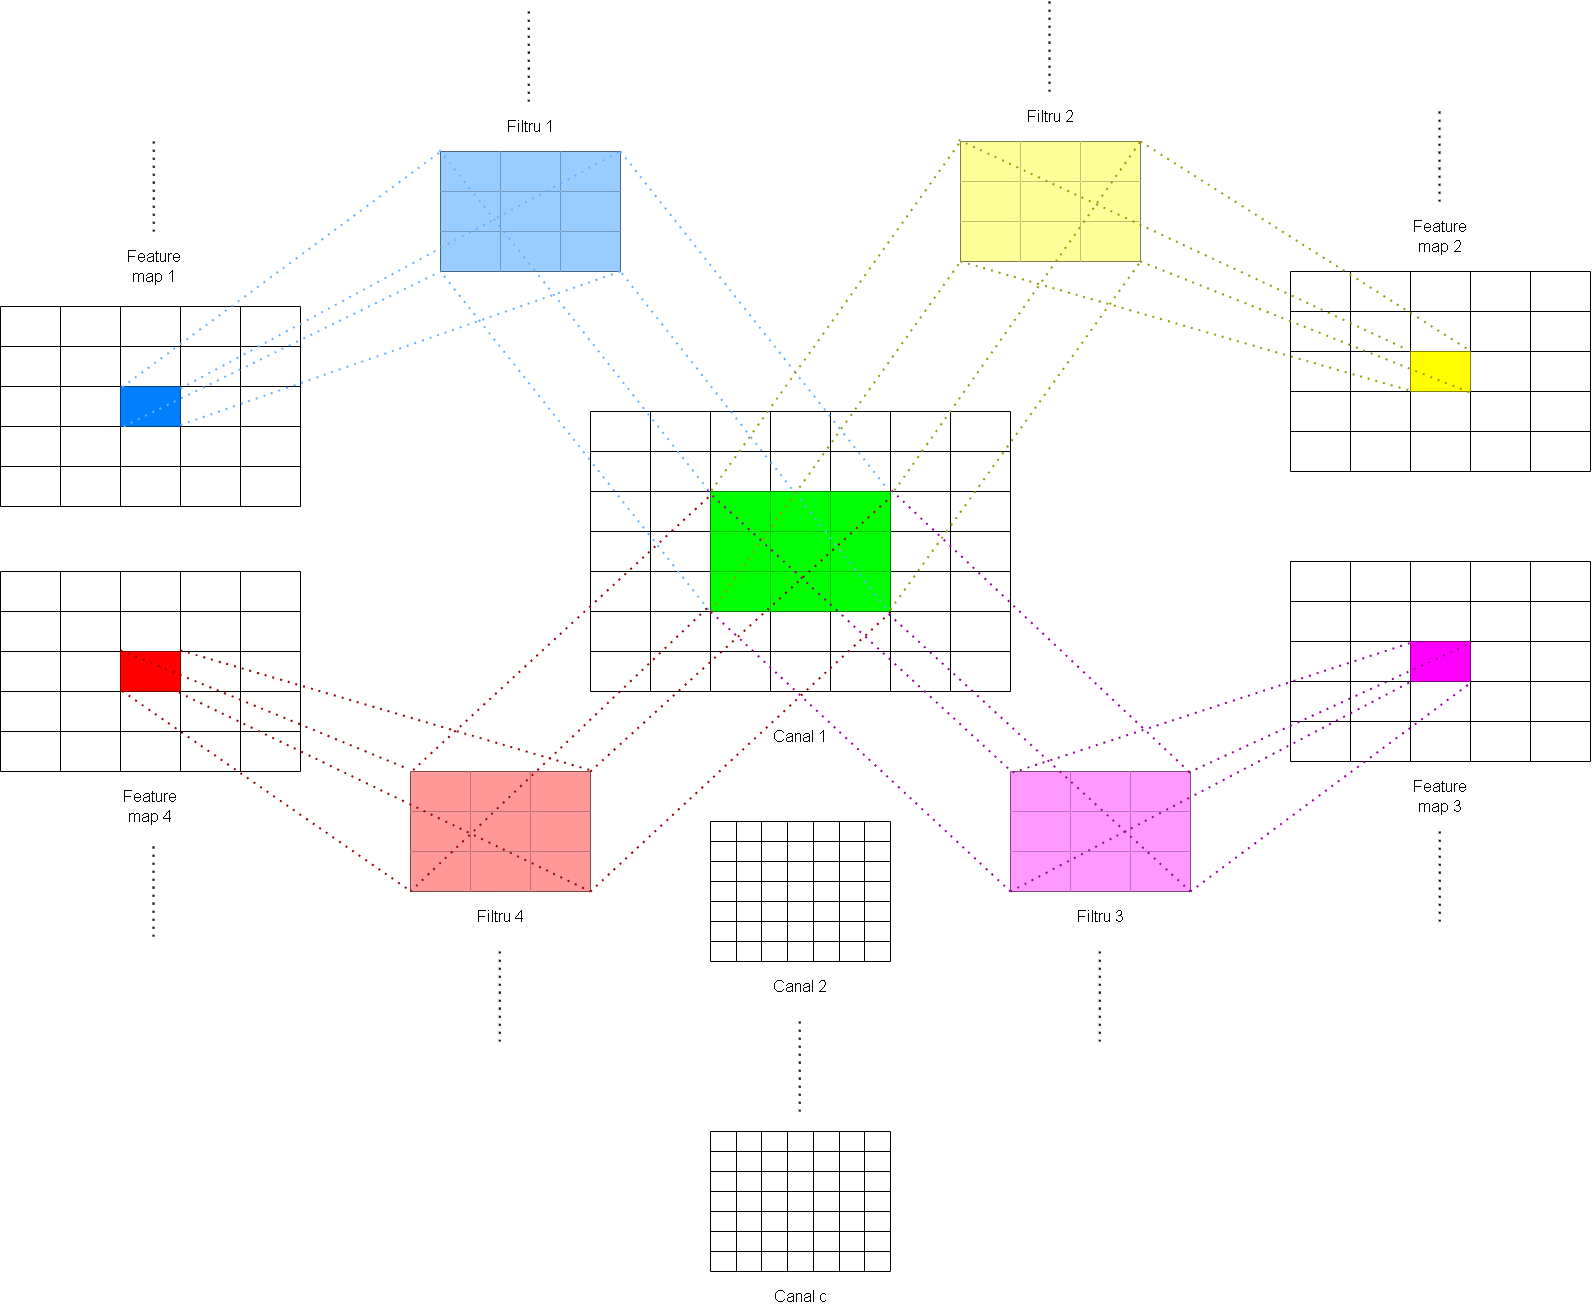
\includegraphics[width=0.7\textwidth]{figures/2d-csnn.png}
    \caption{Reprezentarea procesului de convoluție 2D.}
    \label{fig:conv2d}
\end{figure}

\subsection*{3D-CSNN pentru procesare video}

Extensia către 3D-CSNN urmează aceeași logică bimodală (învățare vs. testare), dar extinde domeniul de aplicare în dimensiunea temporală. Această arhitectură permite extragerea directă a trăsăturilor spatio-temporale, eliminând necesitatea unor algoritmi externi de calcul al fluxului optic \cite{horn1981determining}.

În etapa de inferență 3D, nucleul glisant integrează informația dintr-un volum de intrare (lățime, înălțime și adâncime temporală), procesul fiind ilustrat în Figura”\ref{fig:conv3d}). Toți neuronii dintr-un volum de ieșire $k$ utilizează același set de ponderi 3D învățate, calculând potențialul de membrană la momentul $t$ conform formulei \eqref{eq:conv3d_spiking}:

\begin{equation}
\label{eq:conv3d_spiking}
V_{m_{x,y,z,k}}(t) = \sum_{i \in E} W_{n(x_i), j(y_i), h(z_i), k_i, k} \cdot f_s(t - t_i),
\end{equation}
unde $h(z_i)$ mapează coordonata temporală a impulsului în fereastra nucleului 3D. Acest mecanism permite neuronilor să devină selectivi la schimbări dinamice, simulând comportamentul neuronilor din cortexul vizual primar care răspund la direcții specifice de mișcare în câmpul receptiv.

\begin{figure}[htbp]
    \centering
    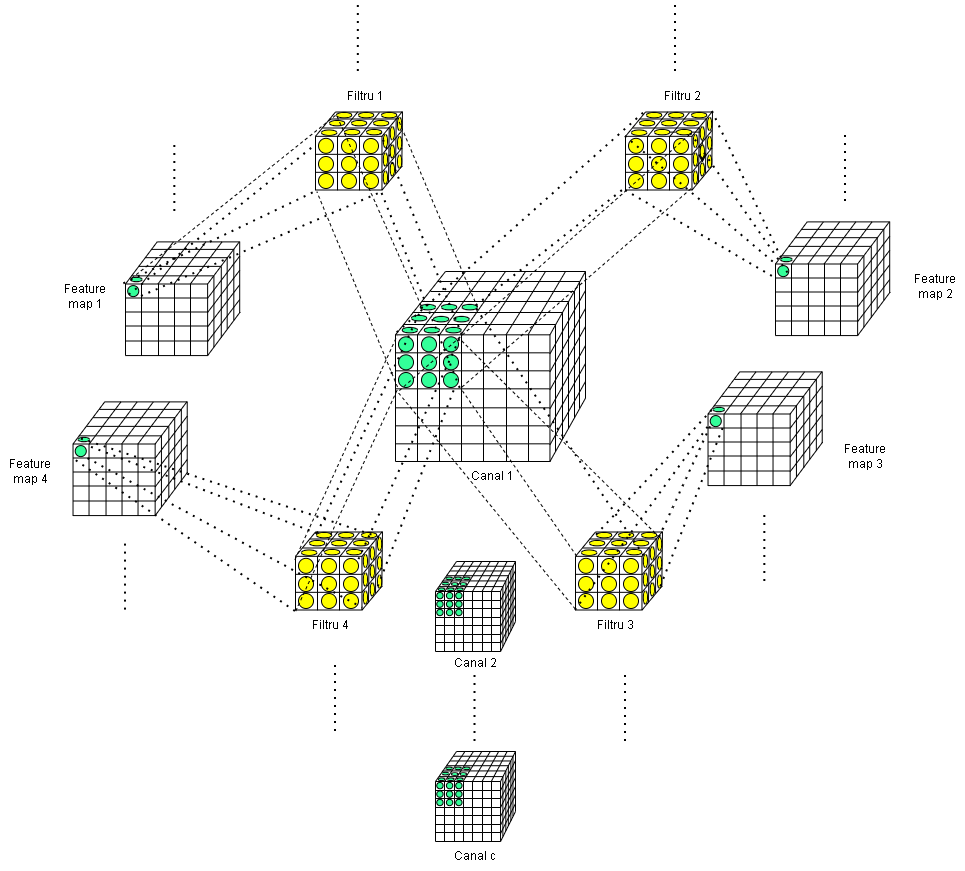
\includegraphics[width=0.75\textwidth]{figures/3d-csnn.png}
    \caption{Operația de convoluție 3D. Aceasta procesează „cuburi” de evenimente, unde aceeași matrice de ponderi $W$ este utilizată pentru a scana întregul flux video.}
    \label{fig:conv3d}
\end{figure}



\section{Metode de eșantionare spațio-temporală a datelor de intrare}
\label{sc:sampling}

În cadrul arhitecturilor de tip Convolutional Spiking Neural Networks (CSNN) aplicate asupra secvențelor video, procesul de eșantionare (\textit{sampling}) joacă un rol critic în eficiența procesării informației vizuale din cadrul etapei de învățare. Spre deosebire de rețelele convoluționale clasice, unde întreaga secvență video este procesată uniform, simulatoarele de SNN pot utiliza strategii de eșantionare pentru a selecta volume locale (\textit{spatio-temporal patches}) care urmează să fie convertite în trenuri de impulsuri (\textit{spikes}).

Această abordare este inspirată din mecanismele biologice de atenție vizuală, permițând modelului să se concentreze pe regiunile cele mai informative ale scenei și pe modificările acestora în timp, reducând astfel costul computațional și influența zgomotului de fundal. În cadrul acestui simulator, au fost implementate patru strategii principale de eșantionare spațio-temporală (3D), în care selecția datelor are loc simultan pe axele spațiale $(x, y)$ și temporală $(t)$. Rezultatul procesului de eșantionare este un volum de date definit de coordonatele $(x, y, t)$, unde $(x, y)$ reprezintă poziția spațială a ferestrei, iar $t$ momentul de start al secvenței temporale analizate.

\subsection*{Eșantionarea aleatorie}

Metoda de eșantionare aleatorie reprezintă abordarea de bază, în care locația volumului de filtrare este determinată în mod stohastic pe întreaga suprafață spațio-temporală a secvenței de intrare. Coordonatele spațiale ale colțului stânga-sus al ferestrei, $(x, y)$, precum și momentul temporal de start $t$, sunt extrase din distribuții uniforme, respectând constrângerile dimensionale ale videoclipului, după cum reiese din relațiile \eqref{eq:distributii_random}:

\begin{equation}
	\label{eq:distributii_random}
	x \sim \mathcal{U}(0, W - w_f), \quad
	y \sim \mathcal{U}(0, H - h_f), \quad
	t \sim \mathcal{U}(0, T - t_f),
\end{equation}
unde $W$ și $H$ reprezintă lățimea și înălțimea cadrului video, $T$ durata totală a secvenței, iar $w_f$, $h_f$ și $t_f$ dimensiunile filtrului pe axele spațiale și temporală.

\subsection*{Strategii faciale bazate pe bounding box}

Pentru a restrânge spațiul de căutare la regiunea facială (\textit{Region of Interest -- ROI}), se utilizează casete de delimitare (\textit{bounding boxes}) detectate în prealabil. Această abordare reduce probabilitatea eșantionării zonelor irelevante și garantează că volumele extrase conțin informație facială relevantă pentru clasificarea emoțiilor. Pentru fiecare fereastră temporală selectată, se calculează o regiune de reuniune (\textit{Union Bounding Box}) care include toate casetele de delimitare asociate cadrelor din intervalul temporal: [$t$, $t+t_f$]. Prin această strategie se garantează faptul că, indiferent de mișcarea capului în cadrul secvenței analizate, volumul extras va conține în permanență regiunea facială a subiectului.

\subsection*{Eșantionarea bazată pe landmark-uri faciale}

Această metodă bazată pe puncte de reper faciale (\textit{facial landmarks}) se fundamentează pe ipoteza că emoțiile feței sunt reprezentate predominant prin variațiile micro-expresiilor localizate în jurul ochilor, sprâncenelor, nasului și gurii. În loc să selecteze volume în mod arbitrar, metoda prioritizează regiunile cu densitate in\-for\-ma\-țio\-na\-lă ridicată, imitând mecanismele biologice ale sistemului vizual uman.

Selecția punctelor de reper urmează schema standard de adnotare cu 68 de land\-mark-uri propusă în setul de date 300-W \cite{sagonas2013300w}, utilizată extensiv în biblioteci precum Dlib sau MediaPipe. Reprezentarea acestor puncte de reper faciale este ilustrată în Figura~\ref{fig:landmarks_68}, iar distribuția lor este prezentată în Tabela~\ref{tab:landmarks}.

\begin{figure}[htbp]
	\centering
	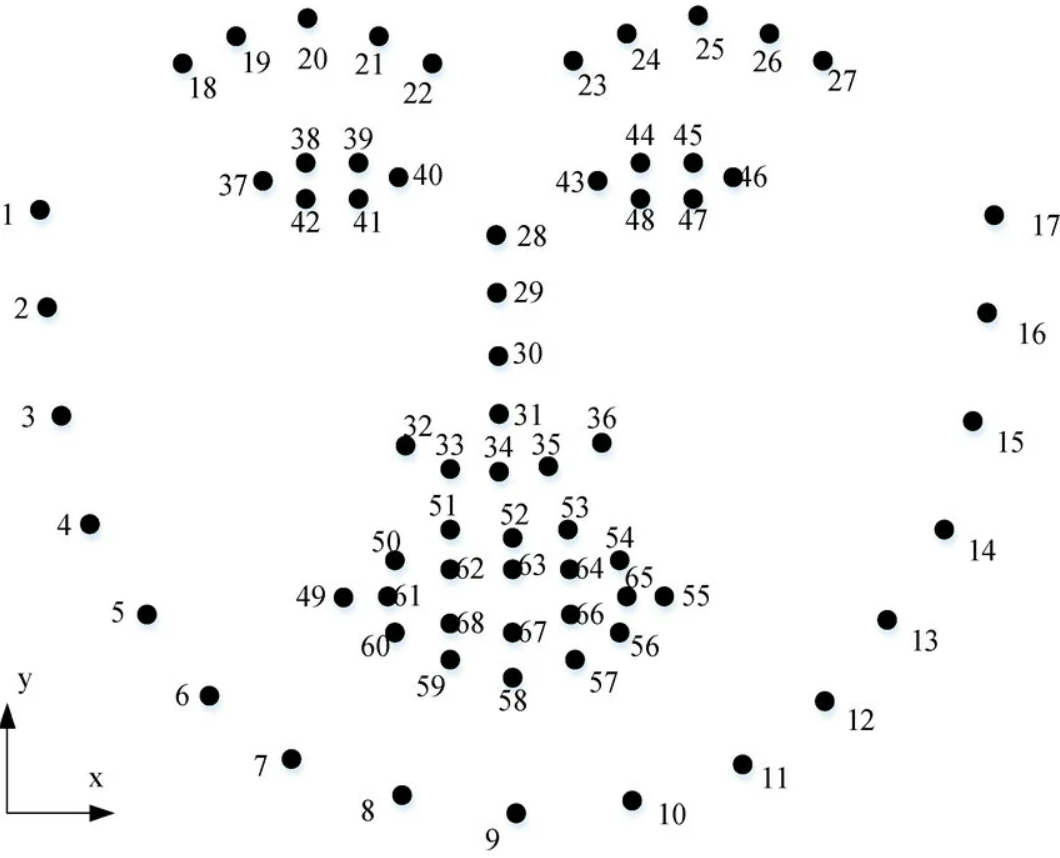
\includegraphics[width=0.7\textwidth]{figures/landmarks_68.png}
	\caption{Reprezentarea celor 68 de puncte de reper faciale (\textit{landmarks}) conform standardului 300-W \cite{li2019}.}
	\label{fig:landmarks_68}
\end{figure}

\begin{table}[h]
	\centering
	\caption{Distribuția punctelor de reper faciale în formatul standard de 68 de puncte.}
	\label{tab:landmarks}
	\begin{tabular}{|l|l|}
		\hline
		\textbf{Regiune Facială} & \textbf{Indici (0-indexed)} \\ \hline
		Contur Mandibulă         & 0 -- 16                     \\ \hline
		Sprânceana Dreaptă       & 17 -- 21                    \\ \hline
		Sprânceana Stângă        & 22 -- 26                    \\ \hline
		Puntea Nazală            & 27 -- 30                    \\ \hline
		Baza Nasului             & 31 -- 35                    \\ \hline
		Ochiul Drept             & 36 -- 41                    \\ \hline
		Ochiul Stâng             & 42 -- 47                    \\ \hline
		Contur Exterior Gură     & 48 -- 59                    \\ \hline
		Contur Interior Gură     & 60 -- 67                    \\ \hline
	\end{tabular}
\end{table}

În cadrul implementării, intervalul de indici $[17, 67]$ este selectat pentru a exclude conturul mandibulei (\textit{jawline}), considerat mai puțin relevant pentru exprimarea emoțiilor, și pentru a maximiza probabilitatea eșantionării trăsăturilor faciale cu valoare semantică ridicată.

Logica algoritmică a metodei presupune parcurgerea mai multor etape. Procedura de eșantionare începe prin selectarea uniformă a unui moment de start $t$ din secvența de intrare. Un punct de reper este apoi ales aleatoriu din subsetul expresiv $[17, 67]$, iar fereastra de extracție spațială de dimensiunea $w_f \times h_f$ este centrată pe coordonatele reperului selectat. Pentru a îmbunătăți robustețea structurală și a reduce \textit{overfittingul}, se introduce o mică perturbație uniformă aleatorie a coordonatelor (\textit{jitter}) în intervalul $[-2, 2]$ pixeli. În cele din urmă, se aplică funcții de \textit{clamping } pentru a se asigura că regiunea extrasă rămâne în limitele video valide.

Această strategie permite rețelei CSNN să urmărească evoluția temporală a unei trăsături faciale specifice (de exemplu curbura gurii în timpul unui zâmbet sau modificările subtile din jurul ochilor asociate expresiilor emoționale) fără necesitatea procesării întregului cadru video.

\subsection*{Eșantionarea bazată pe filtrul ON/OFF}

A patra strategie implementată introduce un mecanism de eșantionare ghidată de relevanță (\textit{saliency-guided sampling}), conceput pentru a prioritiza regiunile spațio-temporale cu activitate neuronală ridicată după aplicarea filtrării de tip DoG și a codificării în impulsuri (\textit{spike encoding}).

Motivația acestei metode pornește de la observația că, în cadrul sistemelor vizuale biologice, atenția este orientată în mod natural către regiunile cu contrast local puternic și variații temporale semnificative. În mod similar, după aplicarea filtrelor ON/OFF de tip DoG, pixelii care prezintă tranziții de intensitate relevante sau modificări expresive subtile generează activitate neuronală mai intensă, reprezentând candidați superiori pentru procesarea ulterioară.

Spre deosebire de strategiile precedente, unde selecția este uniformă sau ghidată geometric, această metodă realizează eșantionarea utilizând o distribuție probabilistică dependentă de relevanța locală a datelor de intrare.

În mod opțional, procesul poate fi restrâns la regiunea facială prin utilizarea casetelor de delimitare (\textit{bounding boxes}), reducând influența fundalului și limitând selecția la zona de interes facială.

Procesul de selecție este realizat în două etape succesive: temporală și spațială.

\subsubsection{Selecția temporală bazată pe relevență}

În prima etapă este determinat momentul temporal $t$ în jurul căruia va fi extras volumul spațio-temporal. Pentru fiecare cadru temporal se calculează un scor global de relevență, obținut prin agregarea activității tuturor pixelilor din regiunea de interes, conform ecuației \eqref{eq:temp_saliency}:

\begin{equation}
	\label{eq:temp_saliency}
	S_t = \sum_{x,y \in ROI} s(x,y,t),
\end{equation}
unde $s(x,y,t)$ reprezintă scorul de relevență asociat pixelului $(x,y)$ la momentul $t$.

În cazul utilizării codificării prin latență (\textit{latency coding}), activitatea neuronală este invers proporțională cu timpul de activare al spike-ului. Astfel, pixelii care generează impulsuri timpurii primesc ponderi mai mari, după cum se poate observa în ecuația \eqref{eq:impuls_latency}.

\begin{equation}
	\label{eq:impuls_latency}
	s(x,y,t)=\max(0,1-v(x,y,t)),
\end{equation}
unde $v(x,y,t)$ reprezintă latența asociată spike-ului. În absența codificării prin latență, scorul este determinat direct din amplitudinea activării.

După calcularea scorurilor temporale, cadrul de interes este selectat utilizând o metodă de tip \textit{roulette wheel selection} (selecție proporțională cu probabilitatea), în care probabilitatea de alegere a unui moment temporal este dată de ecuația \eqref{eq:prob_temp}.

\begin{equation}
	\label{eq:prob_temp}
	P(t)=\frac{S_t}{\sum_k S_k}.
\end{equation}

Prin această formulare, cadrele care conțin activitate neuronală intensă (asociată de regulă mișcărilor faciale subtile sau schimbărilor expresive) au o probabilitate mai mare de a fi selectate.

\subsubsection{Selecția spațială bazată pe relevență}

După determinarea cadrului temporal, procesul continuă prin selecția coordonatelor spațiale $(x,y)$ utilizând aceeași logică probabilistică.

Pentru cadrul selectat, fiecărui pixel din regiunea de interes îi este asociat un scor de relevență, iar probabilitatea de selecție urmează ecuația \eqref{eq:probab_sp}.

\begin{equation}
	\label{eq:probab_sp}
	P(x,y \mid t)=
	\frac{s(x,y,t)}
	{\sum_{i,j \in ROI} s(i,j,t)}.
\end{equation}

Astfel, pixelii care prezintă activitate neuronală ridicată după filtrarea ON/OFF (de exemplu marginile gurii în timpul unui zâmbet sau zona ochilor în expresii de surpriză) au șanse semnificativ mai mari de a deveni centrul volumului eșantionat.

După alegerea punctului central, fereastra spațială de dimensiune $w_f \times h_f$ este poziționată astfel încât pixelul selectat să fie centrat în interiorul acesteia. Ulterior, se aplică o operație de \textit{clamping} pentru a garanta că volumul rezultat rămâne în limitele valide ale secvenței video.

\subsubsection{Mecanism de explorare}

Pentru a evita supra-specializarea modelului asupra acelorași regiuni relevente și pentru a menține diversitatea eșantioanelor, metoda introduce un mecanism explicit de explorare (\textit{exploration factor}).

Cu o probabilitate controlată de parametrul $\alpha \in [0,1]$, denumit factor de explorare (\textit{random mix}), selecția ghidată de relevență este ignorată, iar volumul este extras prin eșantionare aleatorie uniformă: $(x,y,t) \sim \mathcal{U}$.

Această combinație între exploatare (\textit{exploitation}) - focalizarea pe regiunile cu relevență ridicată - și explorare (\textit{exploration}) permite modelului să evite convergența prematură către un set limitat de trăsături și îmbunătățește robustețea generalizării.

În ansamblu, strategia de eșantionare bazată pe relevența ON/OFF oferă un compromis între eficiența computațională și relevanța semantică a informației procesate, direcționând activitatea neuronală către regiunile care conțin cele mai puternice semnale expresive după filtrarea biologic inspirată de tip DoG.

\section{Metode de decodificare a semnalelor neuronale}
În cadrul arhitecturilor de tip Spiking Neural Networks (SNN), etapa de decodificare reprezintă puntea de legătură între activitatea neuronală discretă (spike-uri) și interpretarea acestora sub formă de clase de ieșire (cum ar fi probabilitățile asociate expresiilor faciale). În cazul în care informația în cadrul unei rețele convoluționale cu spike-uri (CSNN) este codificată temporal, relevanța unui impuls depinde direct de momentul apariției sale. Din acest punct de vedere, în literatura de specialitate se pot distinge trei strategii principale de ponderare a activității neuronale. Acestea evaluează importanța spike-urilor în raport cu parametrul de referință $t_{obj}$, ce indică momentul estimat pentru declanșarea nucleului (\textit{kernel}). O valoare ridicată a acestui prag impune integrarea unui număr mai mare de impulsuri pentru declanșare, în timp ce o valoare scăzută reduce această cerință computatională. Comportamentul general al celor trei funcții de decodificare este ilustrat schematic în Figura \ref{fig:metode_decoding}.

\begin{figure}[htbp]
    \centering
    \begin{subfigure}[b]{0.32\textwidth}
        \centering
        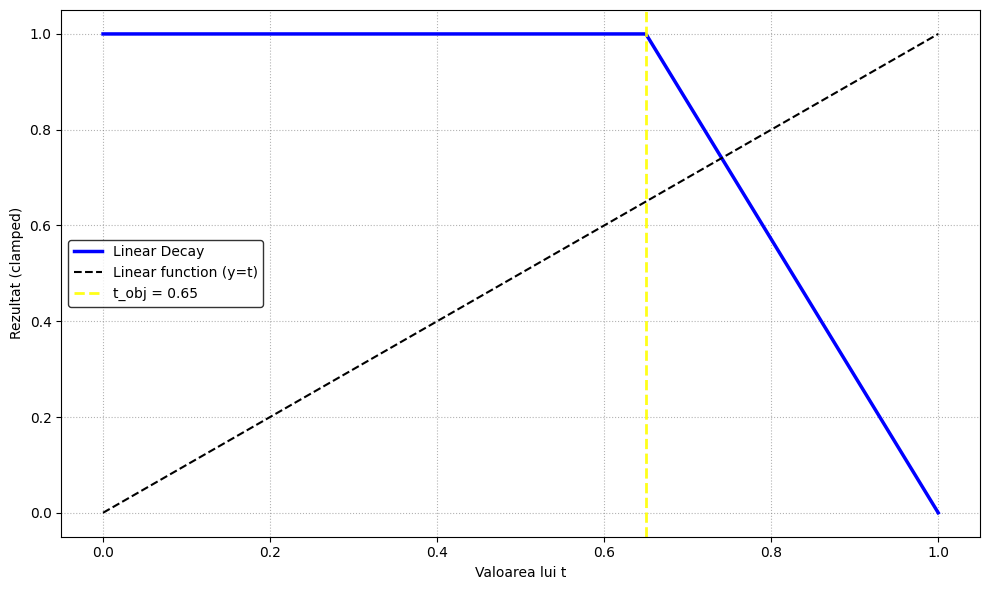
\includegraphics[width=\textwidth]{figures/linear_decay_decoding.png}
        \caption{Linear Decay}
        \label{fig:linear}
    \end{subfigure}
    \hfill
    \begin{subfigure}[b]{0.32\textwidth}
        \centering
        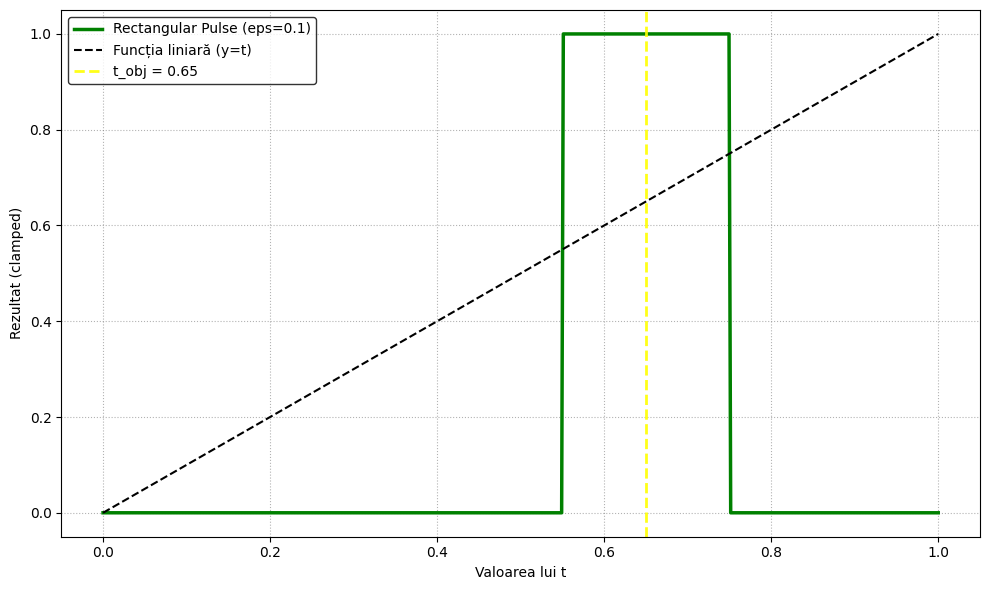
\includegraphics[width=\textwidth]{figures/rectangular_pulse_decoding.png}
        \caption{Rectangular Pulse}
        \label{fig:pulse}
    \end{subfigure}
    \hfill
    \begin{subfigure}[b]{0.32\textwidth}
        \centering
        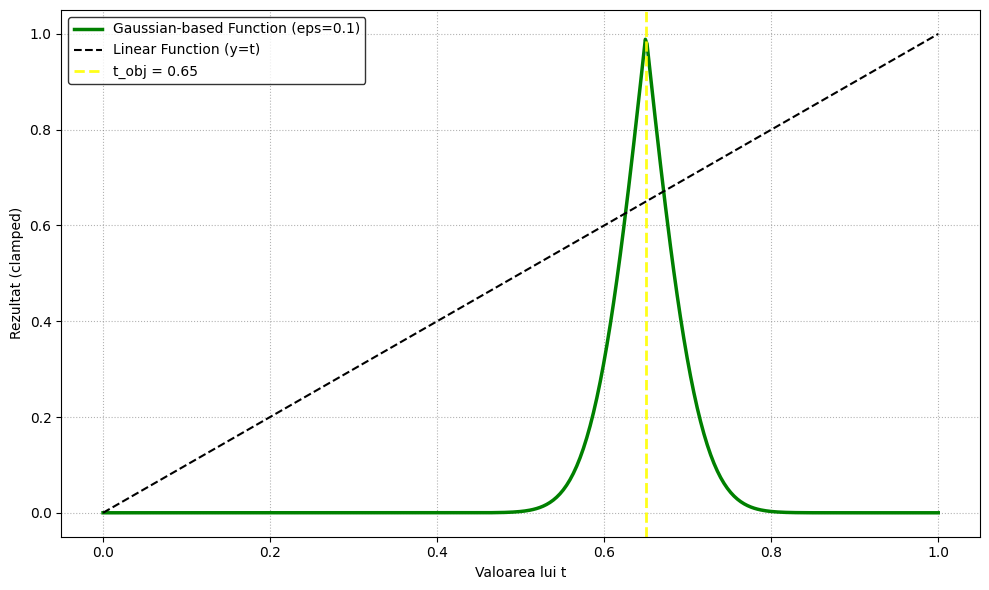
\includegraphics[width=\textwidth]{figures/gaussian-based-decoding.png}
        \caption{Gaussian-based}
        \label{fig:gaussian}
    \end{subfigure}
    \caption{Vizualizarea comparativă a funcțiilor de decodificare utilizate.}
    \label{fig:metode_decoding}
\end{figure}

\subsection*{Decodificarea Linear Decay}
\label{subsection:linear_decay}
Această metodă, ilustrată în Figura \ref{fig:linear}, aplică o descreștere constantă a importanței semnalului pe măsură ce timpul $t$ avansează dincolo de pragul $t_{obj}$. Ea a fost selectată pentru eficiența sa computațională și pentru capacitatea de a modela degradarea simplă a memoriei pe termen scurt a neuronilor, oferind o penalizare proporțională pentru spike-urile care apar târziu în fereastra de procesare a expresiei faciale.

\subsection*{Decodificarea Rectangular Pulse}
Metoda Rectangular Pulse (Figura \ref{fig:pulse}) acționează ca un filtru binar de tip "fereastră". Aceasta atribuie o importanță maximă (1.0) tuturor spike-urilor care apar într-un interval strict de $\pm 0.1$ față de centrul $t_{obj}$, ignorând complet restul activității. Această abordare este utilă pentru detectarea coincidențelor temporale rigide, eliminând zgomotul de fond și spike-urile izolate care nu se încadrează în dinamica temporală specifică unei anumite micro-expresii.

\subsection*{Decodificarea gaussiană (Gaussian-based Importance)}
Cea mai sofisticată metodă, bazată pe funcția de eroare ($\text{erf}$), generează o curbă de tip clopot centrată pe $t_{obj}$ (Figura \ref{fig:gaussian}). Spre deosebire de metodele anterioare, aceasta aproximează cel mai bine variabilitatea biologică a neuronilor și oferă o tranziție lină (smooth transition), fiind robustă la mici variații temporale.

\section*{Concluzii}
Acest capitol a oferit o analiză riguroasă a fundamentelor teoretice, marcând tranziția de la algoritmii clasici de învățare automată și rețelele din a doua generație (CNN, LSTM) către paradigma neuromorfică a rețelelor cu impulsuri (SNN). Prin detalierea modelului de neuron \textit{Integrate-and-Fire}, a filtrelor bio-inspirate DoG, a strategiilor de codificare neurală și a mecanismelor de plasticitate sinaptică (STDP, auto-inhibiția și homeostazia), s-a conturat un cadru conceptual robust și unitar. Cu aceste noțiuni fundamentale clar definite, sunt asigurate toate premisele necesare pentru implementarea arhitecturii propuse de tip CSNN. În cadrul etapelor următoare, acest ansamblu teoretic va fi transpus într-un pipeline experimental aplicat pe sec\-ven\-țe\-le video din setul de date CK+, permițând evaluarea sistematică și validarea comparativă atât a performanței diverselor scheme de eșantionare spațio-temporală (3D sampling), cât și a mai multor tipuri de arhitecturi în sarcina de re\-cu\-noaș\-te\-re a expresiilor faciale.